\section{Background}
    An out of order execution system has two additional stages 
to the lifetime of the instruction on top of the traditional pipeline 
stages.  Each of which is a small memory array to keep track of instruction flow.
The first addition, the instruction queue(IQ), holds instructions that are 
waiting to be executed.  Each entry will hold the instruction -- including 
type, operand registers, and destination registers.  The second structure 
(ROB) holds the instructions that are in flight but not yet committed to the register
file. Each entry will hold both PC of the instruction, as well as the destination
register and the result of the execution unit.  There is also a flag that will
mark the result of the entry as valid.  

Replacing the traditional instruction dispatch stage, a placeholder will be made for the
instruction in reorder buffer and the instructions will be placed
in the instruction queue(IQ). In this stage instructions will first wait for their operands if not already
available.  When all operands are available, the instruction is ready to
be executed and waits until its appropriate execution unit is free.  At this
point the instruction exits the IQ and begins execution.

Upon execution completion, the output value is stored in the ROB with its 
corresponding entry and that entry is marked as valid or completed with a 
1 bit flag.  An entry is committed from the ROB to the architectural register
file (ARF) when that entry is the oldest (lowest PC) and its result has been 
marked as valid. 
\subsection{Circular ROB}
The circular ROB is one of the most basic implementations of the ROB.  It is implemented simply using
a circular buffer as the structure to hold each ROB entry.  Since the ROB is basically
just memory, there are two special slots to keep track of the head and tail
pointers of the circular buffer.  As entries are written into the ROB, the
entry is written at the tail pointer and then the tail pointer is incremented.
Likewise when a entry is written to the ARF, the head pointer is incremented.
The circular buffer method is widely used since it inherently keeps track of the 
oldest instruction (which is at the head pointer), as well as which entry slots
are used or empty.   However it may not be very power efficient if there is a large
number of empty slots at any given point of the execution.    

\subsection{Dynamic ROB}

The dynamic ROB aims to reduce power usage by turning off portions of the buffer when they are not needed, and turning them back on when they become necessary. By partitioning the buffer into what is essentially smaller buffers, the complexity of each partition is reduced. Further, the ROB will then be custom sized to need, thus reducing energy wasted powering large stretches of empty entries. Due to the large percentage of energy consumption stemming from leakage power, turning off partitions contribute significant power savings over the base circular ROB.

Downsizing the ROB is based on a periodic sampling of the buffer state. A number of cycles, {\it update\_period}, is defined, and every {\it update\_period} cycles the size of the ROB is updated. Every {\it sample\_period} cycles, the number of active entries is recorded, and the quantity {\it active\_size} is recorded as the average of these samples between each {\it update\_period}. The current maximum capacity of the reorder buffer is defined as the {\it current\_size}, and the size of a single ROB partition is defined as {\it partition\_size}. After each {\it update\_period} cycles, the ROB checks how full the buffer is, and if {\it current\_size} - {\it active\_size} > {\it partition\_size}, then a single partition is turned off.

Increasing the size of the ROB is dependent on how often the buffer fills up. A value, defined as the {\it overflow\_count} is incremented each cycle that instruction issue is stalled because the ROB is full. An {\it overflow\_threshold} is defined, and if during an {\it update\_period}, {\it overflow\_count} > {\it overflow\_threshold}, then a partition is turned on.

\begin{figure*}
\centering
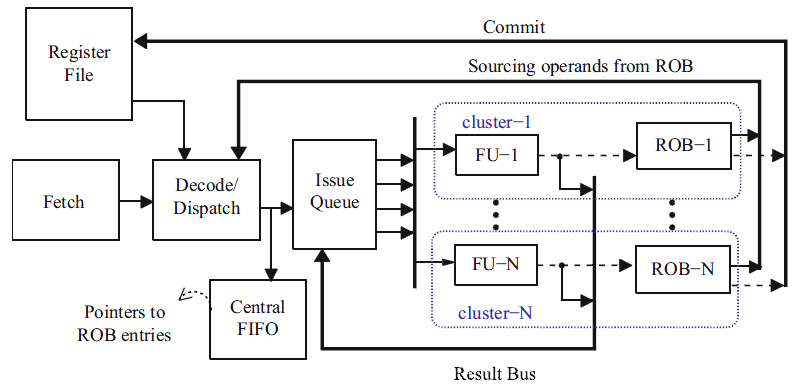
\includegraphics[height=2in]{clusterROB.png}
\caption{Distributed ROB layout}
\label{fig:distrob}
\end{figure*}

\subsection{Distributed ROB}
An accepted optimization for improving the power consumption of an ROB unit
is to break up the ROB buffer into clusters \cite{rabaey}.  In this organization shown in Figure ~\ref{fig:distrob},
the in-flight
instruction information is distributed across all of the units and then re-assembled
back into program order after the fact.  The primary advantage of this approach
is that it dramatically lessens the size of the individual ROB units.  This reduces overall
power by reducing the bit line width as well as unit capacitance.



The overhead associated with this scheme is that the addition of a separate FIFO unit
is required to maintain a global state of instruction order between the separate ROB units.
This central FIFO unit is then referenced upon instruction re-order to commit the instructions
in program order.  The contents of the FIFO unit are fairly simple and incur reasonable hardware
overhead.  Each entry needs only contain the PC of the instruction (or some other unique identifier)
and the corresponding ROB unit that houses the placeholder of the instruction as it is in-flight. 
The total ROB bit storage count remains the same from the non-distributed model to the distributed model
as the overall size of the ROB remains the same.  However, the inclusion of the central FIFO queue 
induces some overhead bits that must be considered when analyzing the overall effectiveness of the 
model.  

The distribution or clustering of the ROB unit also inherently induces a minimal performance overhead 
in particular cases.  By breaking the ROB into smaller pieces and distributing the instruction 
data across the unit, the placement of instructions becomes a performance factor.  Typically, a 
distributed ROB model features only a single write port per ROB cluster.  As a result only one operand 
can be forwarded at a time from the ROB.  In the rare case that an instruction requires two operands be 
forwarded from the same ROB cluster a delay of one cycle is imposed while the operands are forwarded 
sequentially.  It is reported, however, that this happens very rarely in practice and induces less than 1\% 
performance degradation \cite{rabaey}.
\subsection{Latch ROB}
In addition to large power requirement to maintain the entries of the ROB, another 
large power consumer is the read ports of the ROB.  The read port of the ROB is used
to forward the results of an entry to the dispatch unit (DU) to use as an operand.
All though forwarding from the ROB occurs about 6\%\cite{kucuk} of all instructions 
in an N way super scalar processor there are 2N ports (to accommodate FP
 instructions) which add unnecessary complexity and power consumption for a small 
percentage of instructions.  It has been proposed by eliminating the read ports 
in the ROB all together, we can reduce energy consumption\cite{kucuk}.

However without read ports, a small window appears where the data cannot be accessed,
starting from when the result is placed in to the ROB until the ROB commits that 
entry to the ARF.  To help mitigate stalls that might happen due to this hole, 
we introduce retention latches.   Retention latches are small memory elements and 
we use them to cache the most recent results that have been written into the ROB.
This way instructions are still able to access the most recently produced results
and not stall.  However if the operand needed is not in the ROB, the stream will 
stall until a commit is made to the ARF, and that result value is forwarded to 
the dispatch unit immediately.

